\documentclass[tikz,border=2pt]{standalone}
\usepackage{amsmath,mathpazo}
\begin{document}
% !TEX encoding = UTF-8 Unicode
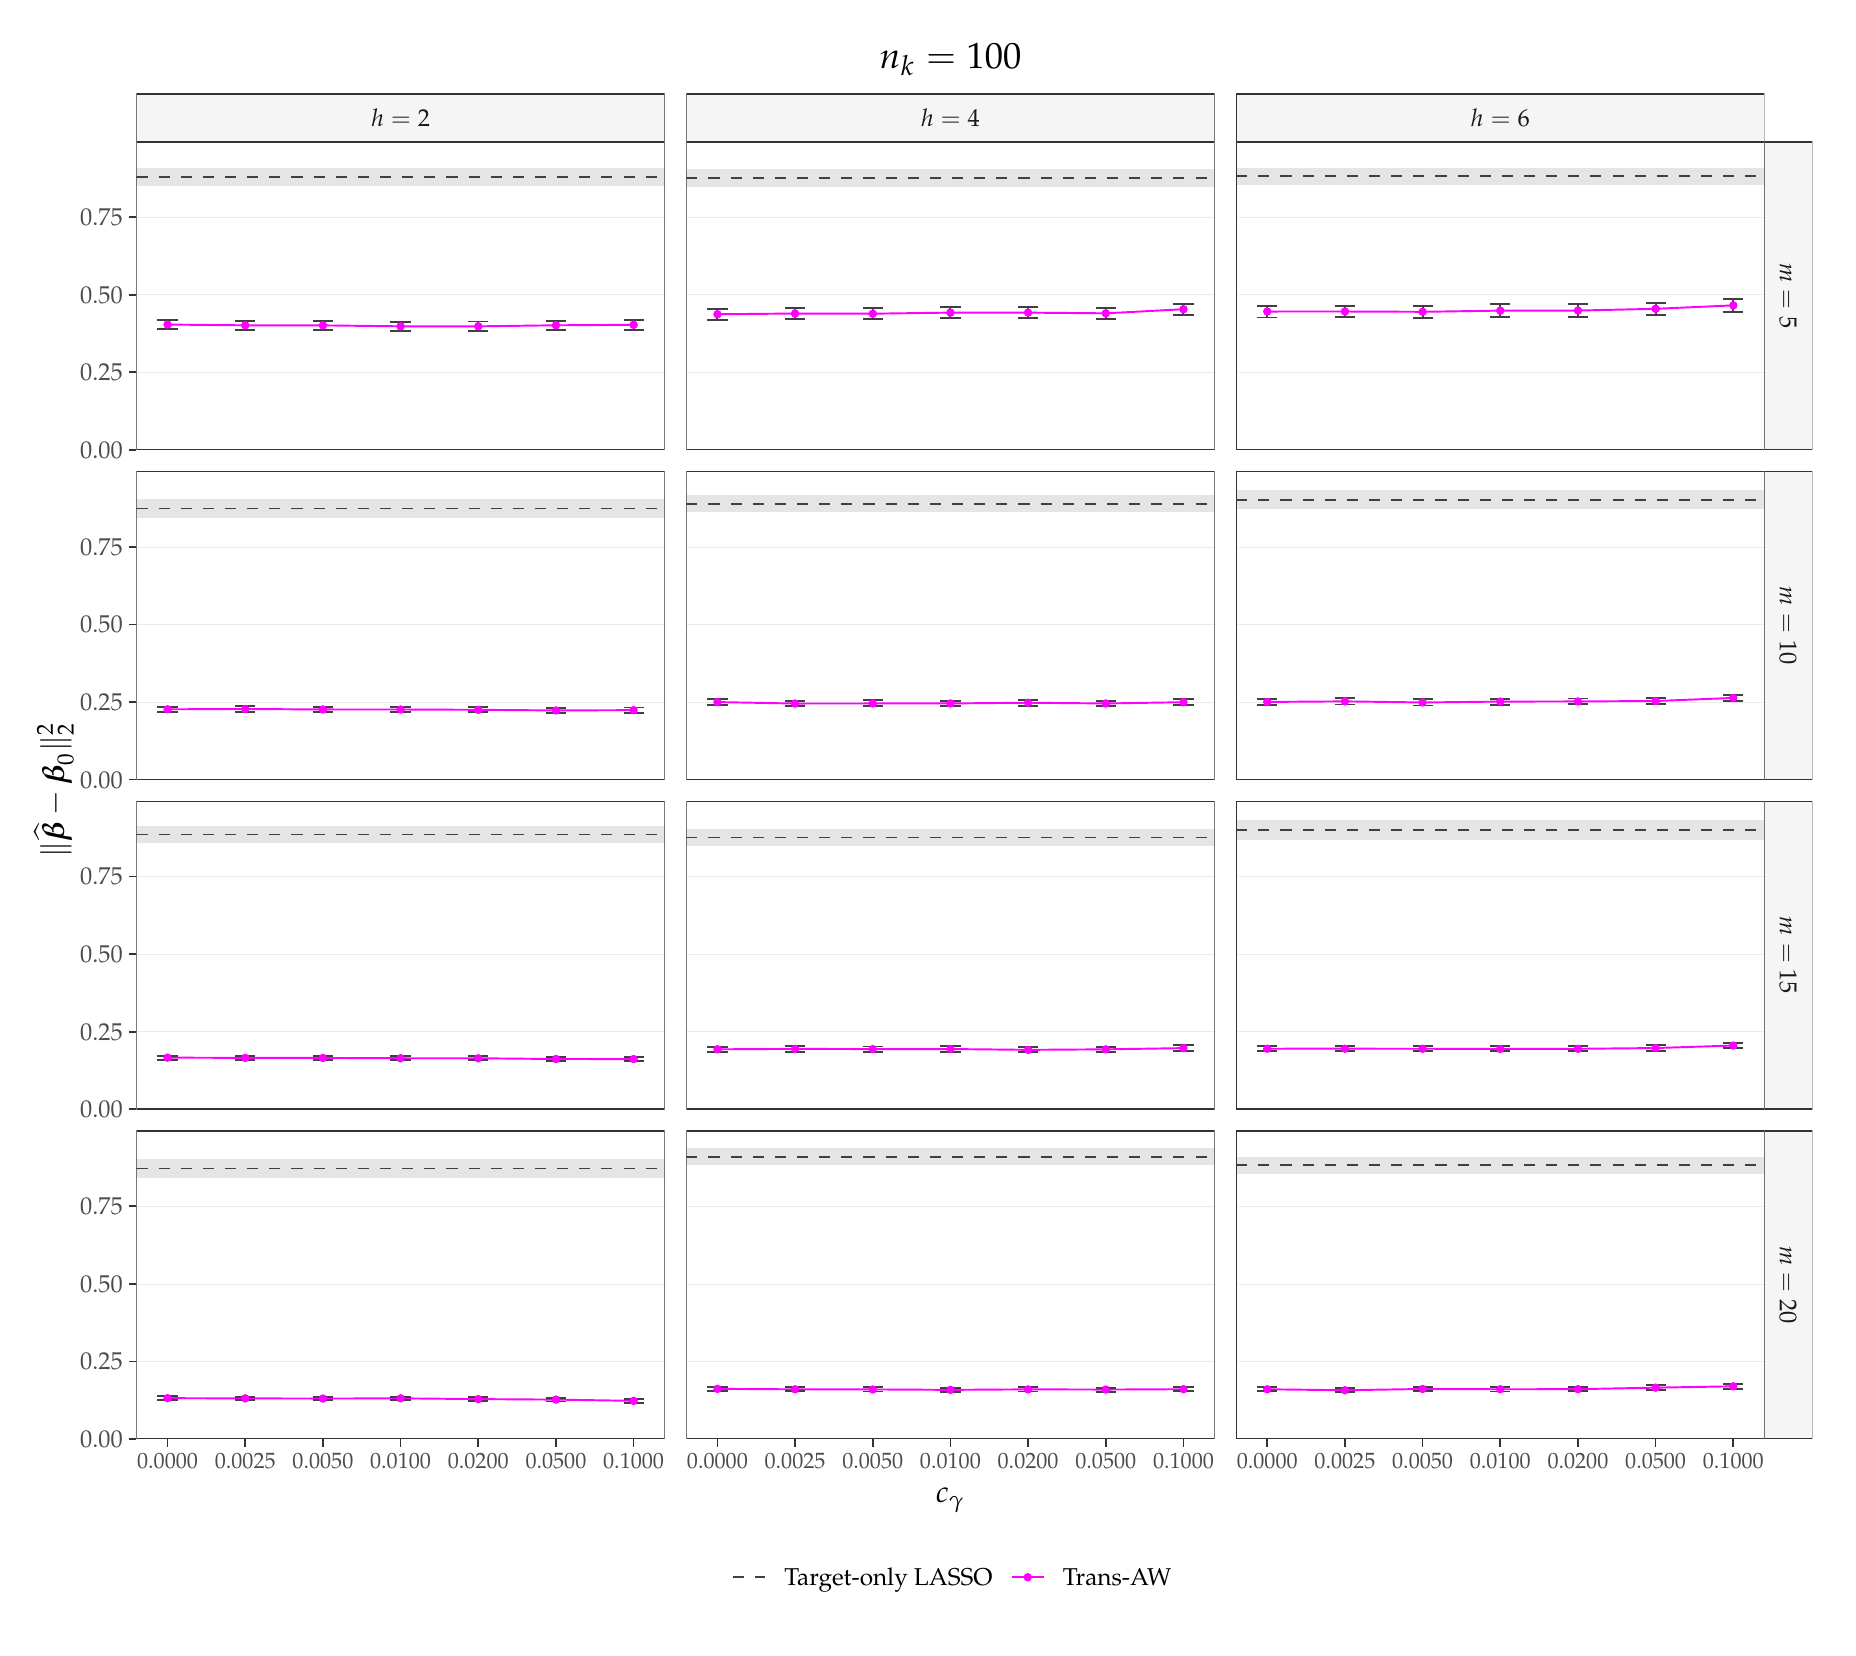
\begin{tikzpicture}[x=1pt,y=1pt]
\definecolor{fillColor}{RGB}{255,255,255}
\path[use as bounding box,fill=fillColor,fill opacity=0.00] (0,0) rectangle (650.43,578.16);
\begin{scope}
\path[clip] (  0.00,  0.00) rectangle (650.43,578.16);
\definecolor{drawColor}{RGB}{255,255,255}
\definecolor{fillColor}{RGB}{255,255,255}

\path[draw=drawColor,line width= 0.6pt,line join=round,line cap=round,fill=fillColor] (  0.00,  0.00) rectangle (650.43,578.16);
\end{scope}
\begin{scope}
\path[clip] ( 39.32,425.60) rectangle (230.18,536.91);
\definecolor{fillColor}{RGB}{255,255,255}

\path[fill=fillColor] ( 39.32,425.60) rectangle (230.18,536.91);
\definecolor{drawColor}{gray}{0.92}

\path[draw=drawColor,line width= 0.2pt,line join=round] ( 39.32,425.60) --
	(230.18,425.60);

\path[draw=drawColor,line width= 0.2pt,line join=round] ( 39.32,453.63) --
	(230.18,453.63);

\path[draw=drawColor,line width= 0.2pt,line join=round] ( 39.32,481.67) --
	(230.18,481.67);

\path[draw=drawColor,line width= 0.2pt,line join=round] ( 39.32,509.70) --
	(230.18,509.70);
\definecolor{fillColor}{gray}{0.90}

\path[fill=fillColor] ( 39.32,521.04) rectangle (230.18,527.37);
\definecolor{drawColor}{gray}{0.25}

\path[draw=drawColor,line width= 0.6pt,dash pattern=on 4pt off 4pt ,line join=round] ( 39.32,524.21) -- (230.18,524.21);
\definecolor{drawColor}{RGB}{255,0,255}

\path[draw=drawColor,line width= 0.7pt,line join=round] ( 50.55,470.87) --
	( 78.62,470.60) --
	(106.69,470.57) --
	(134.75,470.24) --
	(162.82,470.23) --
	(190.89,470.61) --
	(218.95,470.78);
\definecolor{drawColor}{gray}{0.25}

\path[draw=drawColor,line width= 0.7pt,line join=round] ( 46.90,472.55) --
	( 54.20,472.55);

\path[draw=drawColor,line width= 0.7pt,line join=round] ( 50.55,472.55) --
	( 50.55,469.20);

\path[draw=drawColor,line width= 0.7pt,line join=round] ( 46.90,469.20) --
	( 54.20,469.20);

\path[draw=drawColor,line width= 0.7pt,line join=round] ( 74.97,472.31) --
	( 82.27,472.31);

\path[draw=drawColor,line width= 0.7pt,line join=round] ( 78.62,472.31) --
	( 78.62,468.89);

\path[draw=drawColor,line width= 0.7pt,line join=round] ( 74.97,468.89) --
	( 82.27,468.89);

\path[draw=drawColor,line width= 0.7pt,line join=round] (103.04,472.25) --
	(110.33,472.25);

\path[draw=drawColor,line width= 0.7pt,line join=round] (106.69,472.25) --
	(106.69,468.89);

\path[draw=drawColor,line width= 0.7pt,line join=round] (103.04,468.89) --
	(110.33,468.89);

\path[draw=drawColor,line width= 0.7pt,line join=round] (131.10,471.90) --
	(138.40,471.90);

\path[draw=drawColor,line width= 0.7pt,line join=round] (134.75,471.90) --
	(134.75,468.58);

\path[draw=drawColor,line width= 0.7pt,line join=round] (131.10,468.58) --
	(138.40,468.58);

\path[draw=drawColor,line width= 0.7pt,line join=round] (159.17,471.97) --
	(166.47,471.97);

\path[draw=drawColor,line width= 0.7pt,line join=round] (162.82,471.97) --
	(162.82,468.49);

\path[draw=drawColor,line width= 0.7pt,line join=round] (159.17,468.49) --
	(166.47,468.49);

\path[draw=drawColor,line width= 0.7pt,line join=round] (187.24,472.31) --
	(194.54,472.31);

\path[draw=drawColor,line width= 0.7pt,line join=round] (190.89,472.31) --
	(190.89,468.90);

\path[draw=drawColor,line width= 0.7pt,line join=round] (187.24,468.90) --
	(194.54,468.90);

\path[draw=drawColor,line width= 0.7pt,line join=round] (215.31,472.57) --
	(222.60,472.57);

\path[draw=drawColor,line width= 0.7pt,line join=round] (218.95,472.57) --
	(218.95,468.99);

\path[draw=drawColor,line width= 0.7pt,line join=round] (215.31,468.99) --
	(222.60,468.99);
\definecolor{drawColor}{RGB}{255,0,255}
\definecolor{fillColor}{RGB}{255,0,255}

\path[draw=drawColor,line width= 0.4pt,line join=round,line cap=round,fill=fillColor] ( 50.55,470.87) circle (  1.32);

\path[draw=drawColor,line width= 0.4pt,line join=round,line cap=round,fill=fillColor] ( 78.62,470.60) circle (  1.32);

\path[draw=drawColor,line width= 0.4pt,line join=round,line cap=round,fill=fillColor] (106.69,470.57) circle (  1.32);

\path[draw=drawColor,line width= 0.4pt,line join=round,line cap=round,fill=fillColor] (134.75,470.24) circle (  1.32);

\path[draw=drawColor,line width= 0.4pt,line join=round,line cap=round,fill=fillColor] (162.82,470.23) circle (  1.32);

\path[draw=drawColor,line width= 0.4pt,line join=round,line cap=round,fill=fillColor] (190.89,470.61) circle (  1.32);

\path[draw=drawColor,line width= 0.4pt,line join=round,line cap=round,fill=fillColor] (218.95,470.78) circle (  1.32);
\definecolor{drawColor}{gray}{0.20}

\path[draw=drawColor,line width= 0.6pt,line join=round,line cap=round] ( 39.32,425.60) rectangle (230.18,536.91);
\end{scope}
\begin{scope}
\path[clip] ( 39.32,306.46) rectangle (230.18,417.77);
\definecolor{fillColor}{RGB}{255,255,255}

\path[fill=fillColor] ( 39.32,306.46) rectangle (230.18,417.77);
\definecolor{drawColor}{gray}{0.92}

\path[draw=drawColor,line width= 0.2pt,line join=round] ( 39.32,306.46) --
	(230.18,306.46);

\path[draw=drawColor,line width= 0.2pt,line join=round] ( 39.32,334.49) --
	(230.18,334.49);

\path[draw=drawColor,line width= 0.2pt,line join=round] ( 39.32,362.53) --
	(230.18,362.53);

\path[draw=drawColor,line width= 0.2pt,line join=round] ( 39.32,390.56) --
	(230.18,390.56);
\definecolor{fillColor}{gray}{0.90}

\path[fill=fillColor] ( 39.32,401.08) rectangle (230.18,407.66);
\definecolor{drawColor}{gray}{0.25}

\path[draw=drawColor,line width= 0.6pt,dash pattern=on 4pt off 4pt ,line join=round] ( 39.32,404.37) -- (230.18,404.37);
\definecolor{drawColor}{RGB}{255,0,255}

\path[draw=drawColor,line width= 0.7pt,line join=round] ( 50.55,331.85) --
	( 78.62,331.96) --
	(106.69,331.79) --
	(134.75,331.78) --
	(162.82,331.66) --
	(190.89,331.44) --
	(218.95,331.54);
\definecolor{drawColor}{gray}{0.25}

\path[draw=drawColor,line width= 0.7pt,line join=round] ( 46.90,332.76) --
	( 54.20,332.76);

\path[draw=drawColor,line width= 0.7pt,line join=round] ( 50.55,332.76) --
	( 50.55,330.94);

\path[draw=drawColor,line width= 0.7pt,line join=round] ( 46.90,330.94) --
	( 54.20,330.94);

\path[draw=drawColor,line width= 0.7pt,line join=round] ( 74.97,332.89) --
	( 82.27,332.89);

\path[draw=drawColor,line width= 0.7pt,line join=round] ( 78.62,332.89) --
	( 78.62,331.03);

\path[draw=drawColor,line width= 0.7pt,line join=round] ( 74.97,331.03) --
	( 82.27,331.03);

\path[draw=drawColor,line width= 0.7pt,line join=round] (103.04,332.68) --
	(110.33,332.68);

\path[draw=drawColor,line width= 0.7pt,line join=round] (106.69,332.68) --
	(106.69,330.90);

\path[draw=drawColor,line width= 0.7pt,line join=round] (103.04,330.90) --
	(110.33,330.90);

\path[draw=drawColor,line width= 0.7pt,line join=round] (131.10,332.69) --
	(138.40,332.69);

\path[draw=drawColor,line width= 0.7pt,line join=round] (134.75,332.69) --
	(134.75,330.86);

\path[draw=drawColor,line width= 0.7pt,line join=round] (131.10,330.86) --
	(138.40,330.86);

\path[draw=drawColor,line width= 0.7pt,line join=round] (159.17,332.55) --
	(166.47,332.55);

\path[draw=drawColor,line width= 0.7pt,line join=round] (162.82,332.55) --
	(162.82,330.76);

\path[draw=drawColor,line width= 0.7pt,line join=round] (159.17,330.76) --
	(166.47,330.76);

\path[draw=drawColor,line width= 0.7pt,line join=round] (187.24,332.35) --
	(194.54,332.35);

\path[draw=drawColor,line width= 0.7pt,line join=round] (190.89,332.35) --
	(190.89,330.53);

\path[draw=drawColor,line width= 0.7pt,line join=round] (187.24,330.53) --
	(194.54,330.53);

\path[draw=drawColor,line width= 0.7pt,line join=round] (215.31,332.49) --
	(222.60,332.49);

\path[draw=drawColor,line width= 0.7pt,line join=round] (218.95,332.49) --
	(218.95,330.59);

\path[draw=drawColor,line width= 0.7pt,line join=round] (215.31,330.59) --
	(222.60,330.59);
\definecolor{drawColor}{RGB}{255,0,255}
\definecolor{fillColor}{RGB}{255,0,255}

\path[draw=drawColor,line width= 0.4pt,line join=round,line cap=round,fill=fillColor] ( 50.55,331.85) circle (  1.32);

\path[draw=drawColor,line width= 0.4pt,line join=round,line cap=round,fill=fillColor] ( 78.62,331.96) circle (  1.32);

\path[draw=drawColor,line width= 0.4pt,line join=round,line cap=round,fill=fillColor] (106.69,331.79) circle (  1.32);

\path[draw=drawColor,line width= 0.4pt,line join=round,line cap=round,fill=fillColor] (134.75,331.78) circle (  1.32);

\path[draw=drawColor,line width= 0.4pt,line join=round,line cap=round,fill=fillColor] (162.82,331.66) circle (  1.32);

\path[draw=drawColor,line width= 0.4pt,line join=round,line cap=round,fill=fillColor] (190.89,331.44) circle (  1.32);

\path[draw=drawColor,line width= 0.4pt,line join=round,line cap=round,fill=fillColor] (218.95,331.54) circle (  1.32);
\definecolor{drawColor}{gray}{0.20}

\path[draw=drawColor,line width= 0.6pt,line join=round,line cap=round] ( 39.32,306.46) rectangle (230.18,417.77);
\end{scope}
\begin{scope}
\path[clip] ( 39.32,187.32) rectangle (230.18,298.63);
\definecolor{fillColor}{RGB}{255,255,255}

\path[fill=fillColor] ( 39.32,187.32) rectangle (230.18,298.63);
\definecolor{drawColor}{gray}{0.92}

\path[draw=drawColor,line width= 0.2pt,line join=round] ( 39.32,187.32) --
	(230.18,187.32);

\path[draw=drawColor,line width= 0.2pt,line join=round] ( 39.32,215.35) --
	(230.18,215.35);

\path[draw=drawColor,line width= 0.2pt,line join=round] ( 39.32,243.39) --
	(230.18,243.39);

\path[draw=drawColor,line width= 0.2pt,line join=round] ( 39.32,271.42) --
	(230.18,271.42);
\definecolor{fillColor}{gray}{0.90}

\path[fill=fillColor] ( 39.32,283.36) rectangle (230.18,289.74);
\definecolor{drawColor}{gray}{0.25}

\path[draw=drawColor,line width= 0.6pt,dash pattern=on 4pt off 4pt ,line join=round] ( 39.32,286.55) -- (230.18,286.55);
\definecolor{drawColor}{RGB}{255,0,255}

\path[draw=drawColor,line width= 0.7pt,line join=round] ( 50.55,205.98) --
	( 78.62,205.89) --
	(106.69,205.87) --
	(134.75,205.77) --
	(162.82,205.75) --
	(190.89,205.48) --
	(218.95,205.47);
\definecolor{drawColor}{gray}{0.25}

\path[draw=drawColor,line width= 0.7pt,line join=round] ( 46.90,206.71) --
	( 54.20,206.71);

\path[draw=drawColor,line width= 0.7pt,line join=round] ( 50.55,206.71) --
	( 50.55,205.24);

\path[draw=drawColor,line width= 0.7pt,line join=round] ( 46.90,205.24) --
	( 54.20,205.24);

\path[draw=drawColor,line width= 0.7pt,line join=round] ( 74.97,206.62) --
	( 82.27,206.62);

\path[draw=drawColor,line width= 0.7pt,line join=round] ( 78.62,206.62) --
	( 78.62,205.17);

\path[draw=drawColor,line width= 0.7pt,line join=round] ( 74.97,205.17) --
	( 82.27,205.17);

\path[draw=drawColor,line width= 0.7pt,line join=round] (103.04,206.58) --
	(110.33,206.58);

\path[draw=drawColor,line width= 0.7pt,line join=round] (106.69,206.58) --
	(106.69,205.16);

\path[draw=drawColor,line width= 0.7pt,line join=round] (103.04,205.16) --
	(110.33,205.16);

\path[draw=drawColor,line width= 0.7pt,line join=round] (131.10,206.48) --
	(138.40,206.48);

\path[draw=drawColor,line width= 0.7pt,line join=round] (134.75,206.48) --
	(134.75,205.06);

\path[draw=drawColor,line width= 0.7pt,line join=round] (131.10,205.06) --
	(138.40,205.06);

\path[draw=drawColor,line width= 0.7pt,line join=round] (159.17,206.46) --
	(166.47,206.46);

\path[draw=drawColor,line width= 0.7pt,line join=round] (162.82,206.46) --
	(162.82,205.04);

\path[draw=drawColor,line width= 0.7pt,line join=round] (159.17,205.04) --
	(166.47,205.04);

\path[draw=drawColor,line width= 0.7pt,line join=round] (187.24,206.19) --
	(194.54,206.19);

\path[draw=drawColor,line width= 0.7pt,line join=round] (190.89,206.19) --
	(190.89,204.77);

\path[draw=drawColor,line width= 0.7pt,line join=round] (187.24,204.77) --
	(194.54,204.77);

\path[draw=drawColor,line width= 0.7pt,line join=round] (215.31,206.23) --
	(222.60,206.23);

\path[draw=drawColor,line width= 0.7pt,line join=round] (218.95,206.23) --
	(218.95,204.70);

\path[draw=drawColor,line width= 0.7pt,line join=round] (215.31,204.70) --
	(222.60,204.70);
\definecolor{drawColor}{RGB}{255,0,255}
\definecolor{fillColor}{RGB}{255,0,255}

\path[draw=drawColor,line width= 0.4pt,line join=round,line cap=round,fill=fillColor] ( 50.55,205.98) circle (  1.32);

\path[draw=drawColor,line width= 0.4pt,line join=round,line cap=round,fill=fillColor] ( 78.62,205.89) circle (  1.32);

\path[draw=drawColor,line width= 0.4pt,line join=round,line cap=round,fill=fillColor] (106.69,205.87) circle (  1.32);

\path[draw=drawColor,line width= 0.4pt,line join=round,line cap=round,fill=fillColor] (134.75,205.77) circle (  1.32);

\path[draw=drawColor,line width= 0.4pt,line join=round,line cap=round,fill=fillColor] (162.82,205.75) circle (  1.32);

\path[draw=drawColor,line width= 0.4pt,line join=round,line cap=round,fill=fillColor] (190.89,205.48) circle (  1.32);

\path[draw=drawColor,line width= 0.4pt,line join=round,line cap=round,fill=fillColor] (218.95,205.47) circle (  1.32);
\definecolor{drawColor}{gray}{0.20}

\path[draw=drawColor,line width= 0.6pt,line join=round,line cap=round] ( 39.32,187.32) rectangle (230.18,298.63);
\end{scope}
\begin{scope}
\path[clip] ( 39.32, 68.18) rectangle (230.18,179.49);
\definecolor{fillColor}{RGB}{255,255,255}

\path[fill=fillColor] ( 39.32, 68.18) rectangle (230.18,179.49);
\definecolor{drawColor}{gray}{0.92}

\path[draw=drawColor,line width= 0.2pt,line join=round] ( 39.32, 68.18) --
	(230.18, 68.18);

\path[draw=drawColor,line width= 0.2pt,line join=round] ( 39.32, 96.21) --
	(230.18, 96.21);

\path[draw=drawColor,line width= 0.2pt,line join=round] ( 39.32,124.25) --
	(230.18,124.25);

\path[draw=drawColor,line width= 0.2pt,line join=round] ( 39.32,152.28) --
	(230.18,152.28);
\definecolor{fillColor}{gray}{0.90}

\path[fill=fillColor] ( 39.32,162.50) rectangle (230.18,169.41);
\definecolor{drawColor}{gray}{0.25}

\path[draw=drawColor,line width= 0.6pt,dash pattern=on 4pt off 4pt ,line join=round] ( 39.32,165.95) -- (230.18,165.95);
\definecolor{drawColor}{RGB}{255,0,255}

\path[draw=drawColor,line width= 0.7pt,line join=round] ( 50.55, 82.93) --
	( 78.62, 82.85) --
	(106.69, 82.79) --
	(134.75, 82.87) --
	(162.82, 82.59) --
	(190.89, 82.41) --
	(218.95, 81.96);
\definecolor{drawColor}{gray}{0.25}

\path[draw=drawColor,line width= 0.7pt,line join=round] ( 46.90, 83.59) --
	( 54.20, 83.59);

\path[draw=drawColor,line width= 0.7pt,line join=round] ( 50.55, 83.59) --
	( 50.55, 82.27);

\path[draw=drawColor,line width= 0.7pt,line join=round] ( 46.90, 82.27) --
	( 54.20, 82.27);

\path[draw=drawColor,line width= 0.7pt,line join=round] ( 74.97, 83.50) --
	( 82.27, 83.50);

\path[draw=drawColor,line width= 0.7pt,line join=round] ( 78.62, 83.50) --
	( 78.62, 82.21);

\path[draw=drawColor,line width= 0.7pt,line join=round] ( 74.97, 82.21) --
	( 82.27, 82.21);

\path[draw=drawColor,line width= 0.7pt,line join=round] (103.04, 83.41) --
	(110.33, 83.41);

\path[draw=drawColor,line width= 0.7pt,line join=round] (106.69, 83.41) --
	(106.69, 82.16);

\path[draw=drawColor,line width= 0.7pt,line join=round] (103.04, 82.16) --
	(110.33, 82.16);

\path[draw=drawColor,line width= 0.7pt,line join=round] (131.10, 83.52) --
	(138.40, 83.52);

\path[draw=drawColor,line width= 0.7pt,line join=round] (134.75, 83.52) --
	(134.75, 82.22);

\path[draw=drawColor,line width= 0.7pt,line join=round] (131.10, 82.22) --
	(138.40, 82.22);

\path[draw=drawColor,line width= 0.7pt,line join=round] (159.17, 83.22) --
	(166.47, 83.22);

\path[draw=drawColor,line width= 0.7pt,line join=round] (162.82, 83.22) --
	(162.82, 81.95);

\path[draw=drawColor,line width= 0.7pt,line join=round] (159.17, 81.95) --
	(166.47, 81.95);

\path[draw=drawColor,line width= 0.7pt,line join=round] (187.24, 83.10) --
	(194.54, 83.10);

\path[draw=drawColor,line width= 0.7pt,line join=round] (190.89, 83.10) --
	(190.89, 81.72);

\path[draw=drawColor,line width= 0.7pt,line join=round] (187.24, 81.72) --
	(194.54, 81.72);

\path[draw=drawColor,line width= 0.7pt,line join=round] (215.31, 82.64) --
	(222.60, 82.64);

\path[draw=drawColor,line width= 0.7pt,line join=round] (218.95, 82.64) --
	(218.95, 81.29);

\path[draw=drawColor,line width= 0.7pt,line join=round] (215.31, 81.29) --
	(222.60, 81.29);
\definecolor{drawColor}{RGB}{255,0,255}
\definecolor{fillColor}{RGB}{255,0,255}

\path[draw=drawColor,line width= 0.4pt,line join=round,line cap=round,fill=fillColor] ( 50.55, 82.93) circle (  1.32);

\path[draw=drawColor,line width= 0.4pt,line join=round,line cap=round,fill=fillColor] ( 78.62, 82.85) circle (  1.32);

\path[draw=drawColor,line width= 0.4pt,line join=round,line cap=round,fill=fillColor] (106.69, 82.79) circle (  1.32);

\path[draw=drawColor,line width= 0.4pt,line join=round,line cap=round,fill=fillColor] (134.75, 82.87) circle (  1.32);

\path[draw=drawColor,line width= 0.4pt,line join=round,line cap=round,fill=fillColor] (162.82, 82.59) circle (  1.32);

\path[draw=drawColor,line width= 0.4pt,line join=round,line cap=round,fill=fillColor] (190.89, 82.41) circle (  1.32);

\path[draw=drawColor,line width= 0.4pt,line join=round,line cap=round,fill=fillColor] (218.95, 81.96) circle (  1.32);
\definecolor{drawColor}{gray}{0.20}

\path[draw=drawColor,line width= 0.6pt,line join=round,line cap=round] ( 39.32, 68.18) rectangle (230.18,179.49);
\end{scope}
\begin{scope}
\path[clip] (238.01,425.60) rectangle (428.87,536.91);
\definecolor{fillColor}{RGB}{255,255,255}

\path[fill=fillColor] (238.01,425.60) rectangle (428.87,536.91);
\definecolor{drawColor}{gray}{0.92}

\path[draw=drawColor,line width= 0.2pt,line join=round] (238.01,425.60) --
	(428.87,425.60);

\path[draw=drawColor,line width= 0.2pt,line join=round] (238.01,453.63) --
	(428.87,453.63);

\path[draw=drawColor,line width= 0.2pt,line join=round] (238.01,481.67) --
	(428.87,481.67);

\path[draw=drawColor,line width= 0.2pt,line join=round] (238.01,509.70) --
	(428.87,509.70);
\definecolor{fillColor}{gray}{0.90}

\path[fill=fillColor] (238.01,520.51) rectangle (428.87,527.18);
\definecolor{drawColor}{gray}{0.25}

\path[draw=drawColor,line width= 0.6pt,dash pattern=on 4pt off 4pt ,line join=round] (238.01,523.84) -- (428.87,523.84);
\definecolor{drawColor}{RGB}{255,0,255}

\path[draw=drawColor,line width= 0.7pt,line join=round] (249.24,474.60) --
	(277.30,474.86) --
	(305.37,474.80) --
	(333.44,475.19) --
	(361.50,475.18) --
	(389.57,474.94) --
	(417.64,476.41);
\definecolor{drawColor}{gray}{0.25}

\path[draw=drawColor,line width= 0.7pt,line join=round] (245.59,476.55) --
	(252.89,476.55);

\path[draw=drawColor,line width= 0.7pt,line join=round] (249.24,476.55) --
	(249.24,472.65);

\path[draw=drawColor,line width= 0.7pt,line join=round] (245.59,472.65) --
	(252.89,472.65);

\path[draw=drawColor,line width= 0.7pt,line join=round] (273.65,476.80) --
	(280.95,476.80);

\path[draw=drawColor,line width= 0.7pt,line join=round] (277.30,476.80) --
	(277.30,472.92);

\path[draw=drawColor,line width= 0.7pt,line join=round] (273.65,472.92) --
	(280.95,472.92);

\path[draw=drawColor,line width= 0.7pt,line join=round] (301.72,476.70) --
	(309.02,476.70);

\path[draw=drawColor,line width= 0.7pt,line join=round] (305.37,476.70) --
	(305.37,472.91);

\path[draw=drawColor,line width= 0.7pt,line join=round] (301.72,472.91) --
	(309.02,472.91);

\path[draw=drawColor,line width= 0.7pt,line join=round] (329.79,477.15) --
	(337.09,477.15);

\path[draw=drawColor,line width= 0.7pt,line join=round] (333.44,477.15) --
	(333.44,473.24);

\path[draw=drawColor,line width= 0.7pt,line join=round] (329.79,473.24) --
	(337.09,473.24);

\path[draw=drawColor,line width= 0.7pt,line join=round] (357.86,477.08) --
	(365.15,477.08);

\path[draw=drawColor,line width= 0.7pt,line join=round] (361.50,477.08) --
	(361.50,473.28);

\path[draw=drawColor,line width= 0.7pt,line join=round] (357.86,473.28) --
	(365.15,473.28);

\path[draw=drawColor,line width= 0.7pt,line join=round] (385.92,476.87) --
	(393.22,476.87);

\path[draw=drawColor,line width= 0.7pt,line join=round] (389.57,476.87) --
	(389.57,473.01);

\path[draw=drawColor,line width= 0.7pt,line join=round] (385.92,473.01) --
	(393.22,473.01);

\path[draw=drawColor,line width= 0.7pt,line join=round] (413.99,478.36) --
	(421.29,478.36);

\path[draw=drawColor,line width= 0.7pt,line join=round] (417.64,478.36) --
	(417.64,474.46);

\path[draw=drawColor,line width= 0.7pt,line join=round] (413.99,474.46) --
	(421.29,474.46);
\definecolor{drawColor}{RGB}{255,0,255}
\definecolor{fillColor}{RGB}{255,0,255}

\path[draw=drawColor,line width= 0.4pt,line join=round,line cap=round,fill=fillColor] (249.24,474.60) circle (  1.32);

\path[draw=drawColor,line width= 0.4pt,line join=round,line cap=round,fill=fillColor] (277.30,474.86) circle (  1.32);

\path[draw=drawColor,line width= 0.4pt,line join=round,line cap=round,fill=fillColor] (305.37,474.80) circle (  1.32);

\path[draw=drawColor,line width= 0.4pt,line join=round,line cap=round,fill=fillColor] (333.44,475.19) circle (  1.32);

\path[draw=drawColor,line width= 0.4pt,line join=round,line cap=round,fill=fillColor] (361.50,475.18) circle (  1.32);

\path[draw=drawColor,line width= 0.4pt,line join=round,line cap=round,fill=fillColor] (389.57,474.94) circle (  1.32);

\path[draw=drawColor,line width= 0.4pt,line join=round,line cap=round,fill=fillColor] (417.64,476.41) circle (  1.32);
\definecolor{drawColor}{gray}{0.20}

\path[draw=drawColor,line width= 0.6pt,line join=round,line cap=round] (238.01,425.60) rectangle (428.87,536.91);
\end{scope}
\begin{scope}
\path[clip] (238.01,306.46) rectangle (428.87,417.77);
\definecolor{fillColor}{RGB}{255,255,255}

\path[fill=fillColor] (238.01,306.46) rectangle (428.87,417.77);
\definecolor{drawColor}{gray}{0.92}

\path[draw=drawColor,line width= 0.2pt,line join=round] (238.01,306.46) --
	(428.87,306.46);

\path[draw=drawColor,line width= 0.2pt,line join=round] (238.01,334.49) --
	(428.87,334.49);

\path[draw=drawColor,line width= 0.2pt,line join=round] (238.01,362.53) --
	(428.87,362.53);

\path[draw=drawColor,line width= 0.2pt,line join=round] (238.01,390.56) --
	(428.87,390.56);
\definecolor{fillColor}{gray}{0.90}

\path[fill=fillColor] (238.01,402.99) rectangle (428.87,409.22);
\definecolor{drawColor}{gray}{0.25}

\path[draw=drawColor,line width= 0.6pt,dash pattern=on 4pt off 4pt ,line join=round] (238.01,406.10) -- (428.87,406.10);
\definecolor{drawColor}{RGB}{255,0,255}

\path[draw=drawColor,line width= 0.7pt,line join=round] (249.24,334.46) --
	(277.30,333.93) --
	(305.37,333.96) --
	(333.44,333.97) --
	(361.50,334.22) --
	(389.57,333.96) --
	(417.64,334.41);
\definecolor{drawColor}{gray}{0.25}

\path[draw=drawColor,line width= 0.7pt,line join=round] (245.59,335.58) --
	(252.89,335.58);

\path[draw=drawColor,line width= 0.7pt,line join=round] (249.24,335.58) --
	(249.24,333.35);

\path[draw=drawColor,line width= 0.7pt,line join=round] (245.59,333.35) --
	(252.89,333.35);

\path[draw=drawColor,line width= 0.7pt,line join=round] (273.65,334.95) --
	(280.95,334.95);

\path[draw=drawColor,line width= 0.7pt,line join=round] (277.30,334.95) --
	(277.30,332.90);

\path[draw=drawColor,line width= 0.7pt,line join=round] (273.65,332.90) --
	(280.95,332.90);

\path[draw=drawColor,line width= 0.7pt,line join=round] (301.72,335.05) --
	(309.02,335.05);

\path[draw=drawColor,line width= 0.7pt,line join=round] (305.37,335.05) --
	(305.37,332.88);

\path[draw=drawColor,line width= 0.7pt,line join=round] (301.72,332.88) --
	(309.02,332.88);

\path[draw=drawColor,line width= 0.7pt,line join=round] (329.79,334.99) --
	(337.09,334.99);

\path[draw=drawColor,line width= 0.7pt,line join=round] (333.44,334.99) --
	(333.44,332.95);

\path[draw=drawColor,line width= 0.7pt,line join=round] (329.79,332.95) --
	(337.09,332.95);

\path[draw=drawColor,line width= 0.7pt,line join=round] (357.86,335.29) --
	(365.15,335.29);

\path[draw=drawColor,line width= 0.7pt,line join=round] (361.50,335.29) --
	(361.50,333.14);

\path[draw=drawColor,line width= 0.7pt,line join=round] (357.86,333.14) --
	(365.15,333.14);

\path[draw=drawColor,line width= 0.7pt,line join=round] (385.92,335.01) --
	(393.22,335.01);

\path[draw=drawColor,line width= 0.7pt,line join=round] (389.57,335.01) --
	(389.57,332.90);

\path[draw=drawColor,line width= 0.7pt,line join=round] (385.92,332.90) --
	(393.22,332.90);

\path[draw=drawColor,line width= 0.7pt,line join=round] (413.99,335.49) --
	(421.29,335.49);

\path[draw=drawColor,line width= 0.7pt,line join=round] (417.64,335.49) --
	(417.64,333.33);

\path[draw=drawColor,line width= 0.7pt,line join=round] (413.99,333.33) --
	(421.29,333.33);
\definecolor{drawColor}{RGB}{255,0,255}
\definecolor{fillColor}{RGB}{255,0,255}

\path[draw=drawColor,line width= 0.4pt,line join=round,line cap=round,fill=fillColor] (249.24,334.46) circle (  1.32);

\path[draw=drawColor,line width= 0.4pt,line join=round,line cap=round,fill=fillColor] (277.30,333.93) circle (  1.32);

\path[draw=drawColor,line width= 0.4pt,line join=round,line cap=round,fill=fillColor] (305.37,333.96) circle (  1.32);

\path[draw=drawColor,line width= 0.4pt,line join=round,line cap=round,fill=fillColor] (333.44,333.97) circle (  1.32);

\path[draw=drawColor,line width= 0.4pt,line join=round,line cap=round,fill=fillColor] (361.50,334.22) circle (  1.32);

\path[draw=drawColor,line width= 0.4pt,line join=round,line cap=round,fill=fillColor] (389.57,333.96) circle (  1.32);

\path[draw=drawColor,line width= 0.4pt,line join=round,line cap=round,fill=fillColor] (417.64,334.41) circle (  1.32);
\definecolor{drawColor}{gray}{0.20}

\path[draw=drawColor,line width= 0.6pt,line join=round,line cap=round] (238.01,306.46) rectangle (428.87,417.77);
\end{scope}
\begin{scope}
\path[clip] (238.01,187.32) rectangle (428.87,298.63);
\definecolor{fillColor}{RGB}{255,255,255}

\path[fill=fillColor] (238.01,187.32) rectangle (428.87,298.63);
\definecolor{drawColor}{gray}{0.92}

\path[draw=drawColor,line width= 0.2pt,line join=round] (238.01,187.32) --
	(428.87,187.32);

\path[draw=drawColor,line width= 0.2pt,line join=round] (238.01,215.35) --
	(428.87,215.35);

\path[draw=drawColor,line width= 0.2pt,line join=round] (238.01,243.39) --
	(428.87,243.39);

\path[draw=drawColor,line width= 0.2pt,line join=round] (238.01,271.42) --
	(428.87,271.42);
\definecolor{fillColor}{gray}{0.90}

\path[fill=fillColor] (238.01,282.44) rectangle (428.87,288.57);
\definecolor{drawColor}{gray}{0.25}

\path[draw=drawColor,line width= 0.6pt,dash pattern=on 4pt off 4pt ,line join=round] (238.01,285.50) -- (428.87,285.50);
\definecolor{drawColor}{RGB}{255,0,255}

\path[draw=drawColor,line width= 0.7pt,line join=round] (249.24,208.99) --
	(277.30,209.14) --
	(305.37,209.07) --
	(333.44,209.09) --
	(361.50,208.79) --
	(389.57,208.98) --
	(417.64,209.42);
\definecolor{drawColor}{gray}{0.25}

\path[draw=drawColor,line width= 0.7pt,line join=round] (245.59,209.89) --
	(252.89,209.89);

\path[draw=drawColor,line width= 0.7pt,line join=round] (249.24,209.89) --
	(249.24,208.09);

\path[draw=drawColor,line width= 0.7pt,line join=round] (245.59,208.09) --
	(252.89,208.09);

\path[draw=drawColor,line width= 0.7pt,line join=round] (273.65,210.10) --
	(280.95,210.10);

\path[draw=drawColor,line width= 0.7pt,line join=round] (277.30,210.10) --
	(277.30,208.18);

\path[draw=drawColor,line width= 0.7pt,line join=round] (273.65,208.18) --
	(280.95,208.18);

\path[draw=drawColor,line width= 0.7pt,line join=round] (301.72,210.00) --
	(309.02,210.00);

\path[draw=drawColor,line width= 0.7pt,line join=round] (305.37,210.00) --
	(305.37,208.14);

\path[draw=drawColor,line width= 0.7pt,line join=round] (301.72,208.14) --
	(309.02,208.14);

\path[draw=drawColor,line width= 0.7pt,line join=round] (329.79,210.02) --
	(337.09,210.02);

\path[draw=drawColor,line width= 0.7pt,line join=round] (333.44,210.02) --
	(333.44,208.17);

\path[draw=drawColor,line width= 0.7pt,line join=round] (329.79,208.17) --
	(337.09,208.17);

\path[draw=drawColor,line width= 0.7pt,line join=round] (357.86,209.69) --
	(365.15,209.69);

\path[draw=drawColor,line width= 0.7pt,line join=round] (361.50,209.69) --
	(361.50,207.88);

\path[draw=drawColor,line width= 0.7pt,line join=round] (357.86,207.88) --
	(365.15,207.88);

\path[draw=drawColor,line width= 0.7pt,line join=round] (385.92,209.90) --
	(393.22,209.90);

\path[draw=drawColor,line width= 0.7pt,line join=round] (389.57,209.90) --
	(389.57,208.06);

\path[draw=drawColor,line width= 0.7pt,line join=round] (385.92,208.06) --
	(393.22,208.06);

\path[draw=drawColor,line width= 0.7pt,line join=round] (413.99,210.38) --
	(421.29,210.38);

\path[draw=drawColor,line width= 0.7pt,line join=round] (417.64,210.38) --
	(417.64,208.46);

\path[draw=drawColor,line width= 0.7pt,line join=round] (413.99,208.46) --
	(421.29,208.46);
\definecolor{drawColor}{RGB}{255,0,255}
\definecolor{fillColor}{RGB}{255,0,255}

\path[draw=drawColor,line width= 0.4pt,line join=round,line cap=round,fill=fillColor] (249.24,208.99) circle (  1.32);

\path[draw=drawColor,line width= 0.4pt,line join=round,line cap=round,fill=fillColor] (277.30,209.14) circle (  1.32);

\path[draw=drawColor,line width= 0.4pt,line join=round,line cap=round,fill=fillColor] (305.37,209.07) circle (  1.32);

\path[draw=drawColor,line width= 0.4pt,line join=round,line cap=round,fill=fillColor] (333.44,209.09) circle (  1.32);

\path[draw=drawColor,line width= 0.4pt,line join=round,line cap=round,fill=fillColor] (361.50,208.79) circle (  1.32);

\path[draw=drawColor,line width= 0.4pt,line join=round,line cap=round,fill=fillColor] (389.57,208.98) circle (  1.32);

\path[draw=drawColor,line width= 0.4pt,line join=round,line cap=round,fill=fillColor] (417.64,209.42) circle (  1.32);
\definecolor{drawColor}{gray}{0.20}

\path[draw=drawColor,line width= 0.6pt,line join=round,line cap=round] (238.01,187.32) rectangle (428.87,298.63);
\end{scope}
\begin{scope}
\path[clip] (238.01, 68.18) rectangle (428.87,179.49);
\definecolor{fillColor}{RGB}{255,255,255}

\path[fill=fillColor] (238.01, 68.18) rectangle (428.87,179.49);
\definecolor{drawColor}{gray}{0.92}

\path[draw=drawColor,line width= 0.2pt,line join=round] (238.01, 68.18) --
	(428.87, 68.18);

\path[draw=drawColor,line width= 0.2pt,line join=round] (238.01, 96.21) --
	(428.87, 96.21);

\path[draw=drawColor,line width= 0.2pt,line join=round] (238.01,124.25) --
	(428.87,124.25);

\path[draw=drawColor,line width= 0.2pt,line join=round] (238.01,152.28) --
	(428.87,152.28);
\definecolor{fillColor}{gray}{0.90}

\path[fill=fillColor] (238.01,167.03) rectangle (428.87,173.19);
\definecolor{drawColor}{gray}{0.25}

\path[draw=drawColor,line width= 0.6pt,dash pattern=on 4pt off 4pt ,line join=round] (238.01,170.11) -- (428.87,170.11);
\definecolor{drawColor}{RGB}{255,0,255}

\path[draw=drawColor,line width= 0.7pt,line join=round] (249.24, 86.29) --
	(277.30, 86.13) --
	(305.37, 86.08) --
	(333.44, 85.93) --
	(361.50, 86.11) --
	(389.57, 86.04) --
	(417.64, 86.17);
\definecolor{drawColor}{gray}{0.25}

\path[draw=drawColor,line width= 0.7pt,line join=round] (245.59, 87.06) --
	(252.89, 87.06);

\path[draw=drawColor,line width= 0.7pt,line join=round] (249.24, 87.06) --
	(249.24, 85.52);

\path[draw=drawColor,line width= 0.7pt,line join=round] (245.59, 85.52) --
	(252.89, 85.52);

\path[draw=drawColor,line width= 0.7pt,line join=round] (273.65, 86.86) --
	(280.95, 86.86);

\path[draw=drawColor,line width= 0.7pt,line join=round] (277.30, 86.86) --
	(277.30, 85.40);

\path[draw=drawColor,line width= 0.7pt,line join=round] (273.65, 85.40) --
	(280.95, 85.40);

\path[draw=drawColor,line width= 0.7pt,line join=round] (301.72, 86.84) --
	(309.02, 86.84);

\path[draw=drawColor,line width= 0.7pt,line join=round] (305.37, 86.84) --
	(305.37, 85.33);

\path[draw=drawColor,line width= 0.7pt,line join=round] (301.72, 85.33) --
	(309.02, 85.33);

\path[draw=drawColor,line width= 0.7pt,line join=round] (329.79, 86.65) --
	(337.09, 86.65);

\path[draw=drawColor,line width= 0.7pt,line join=round] (333.44, 86.65) --
	(333.44, 85.20);

\path[draw=drawColor,line width= 0.7pt,line join=round] (329.79, 85.20) --
	(337.09, 85.20);

\path[draw=drawColor,line width= 0.7pt,line join=round] (357.86, 86.87) --
	(365.15, 86.87);

\path[draw=drawColor,line width= 0.7pt,line join=round] (361.50, 86.87) --
	(361.50, 85.35);

\path[draw=drawColor,line width= 0.7pt,line join=round] (357.86, 85.35) --
	(365.15, 85.35);

\path[draw=drawColor,line width= 0.7pt,line join=round] (385.92, 86.77) --
	(393.22, 86.77);

\path[draw=drawColor,line width= 0.7pt,line join=round] (389.57, 86.77) --
	(389.57, 85.30);

\path[draw=drawColor,line width= 0.7pt,line join=round] (385.92, 85.30) --
	(393.22, 85.30);

\path[draw=drawColor,line width= 0.7pt,line join=round] (413.99, 86.90) --
	(421.29, 86.90);

\path[draw=drawColor,line width= 0.7pt,line join=round] (417.64, 86.90) --
	(417.64, 85.45);

\path[draw=drawColor,line width= 0.7pt,line join=round] (413.99, 85.45) --
	(421.29, 85.45);
\definecolor{drawColor}{RGB}{255,0,255}
\definecolor{fillColor}{RGB}{255,0,255}

\path[draw=drawColor,line width= 0.4pt,line join=round,line cap=round,fill=fillColor] (249.24, 86.29) circle (  1.32);

\path[draw=drawColor,line width= 0.4pt,line join=round,line cap=round,fill=fillColor] (277.30, 86.13) circle (  1.32);

\path[draw=drawColor,line width= 0.4pt,line join=round,line cap=round,fill=fillColor] (305.37, 86.08) circle (  1.32);

\path[draw=drawColor,line width= 0.4pt,line join=round,line cap=round,fill=fillColor] (333.44, 85.93) circle (  1.32);

\path[draw=drawColor,line width= 0.4pt,line join=round,line cap=round,fill=fillColor] (361.50, 86.11) circle (  1.32);

\path[draw=drawColor,line width= 0.4pt,line join=round,line cap=round,fill=fillColor] (389.57, 86.04) circle (  1.32);

\path[draw=drawColor,line width= 0.4pt,line join=round,line cap=round,fill=fillColor] (417.64, 86.17) circle (  1.32);
\definecolor{drawColor}{gray}{0.20}

\path[draw=drawColor,line width= 0.6pt,line join=round,line cap=round] (238.01, 68.18) rectangle (428.87,179.49);
\end{scope}
\begin{scope}
\path[clip] (436.69,425.60) rectangle (627.55,536.91);
\definecolor{fillColor}{RGB}{255,255,255}

\path[fill=fillColor] (436.69,425.60) rectangle (627.55,536.91);
\definecolor{drawColor}{gray}{0.92}

\path[draw=drawColor,line width= 0.2pt,line join=round] (436.69,425.60) --
	(627.55,425.60);

\path[draw=drawColor,line width= 0.2pt,line join=round] (436.69,453.63) --
	(627.55,453.63);

\path[draw=drawColor,line width= 0.2pt,line join=round] (436.69,481.67) --
	(627.55,481.67);

\path[draw=drawColor,line width= 0.2pt,line join=round] (436.69,509.70) --
	(627.55,509.70);
\definecolor{fillColor}{gray}{0.90}

\path[fill=fillColor] (436.69,521.31) rectangle (627.55,527.58);
\definecolor{drawColor}{gray}{0.25}

\path[draw=drawColor,line width= 0.6pt,dash pattern=on 4pt off 4pt ,line join=round] (436.69,524.45) -- (627.55,524.45);
\definecolor{drawColor}{RGB}{255,0,255}

\path[draw=drawColor,line width= 0.7pt,line join=round] (447.92,475.58) --
	(475.99,475.59) --
	(504.06,475.48) --
	(532.12,475.91) --
	(560.19,475.93) --
	(588.26,476.57) --
	(616.32,477.80);
\definecolor{drawColor}{gray}{0.25}

\path[draw=drawColor,line width= 0.7pt,line join=round] (444.27,477.73) --
	(451.57,477.73);

\path[draw=drawColor,line width= 0.7pt,line join=round] (447.92,477.73) --
	(447.92,473.43);

\path[draw=drawColor,line width= 0.7pt,line join=round] (444.27,473.43) --
	(451.57,473.43);

\path[draw=drawColor,line width= 0.7pt,line join=round] (472.34,477.74) --
	(479.64,477.74);

\path[draw=drawColor,line width= 0.7pt,line join=round] (475.99,477.74) --
	(475.99,473.44);

\path[draw=drawColor,line width= 0.7pt,line join=round] (472.34,473.44) --
	(479.64,473.44);

\path[draw=drawColor,line width= 0.7pt,line join=round] (500.41,477.71) --
	(507.70,477.71);

\path[draw=drawColor,line width= 0.7pt,line join=round] (504.06,477.71) --
	(504.06,473.24);

\path[draw=drawColor,line width= 0.7pt,line join=round] (500.41,473.24) --
	(507.70,473.24);

\path[draw=drawColor,line width= 0.7pt,line join=round] (528.47,478.15) --
	(535.77,478.15);

\path[draw=drawColor,line width= 0.7pt,line join=round] (532.12,478.15) --
	(532.12,473.66);

\path[draw=drawColor,line width= 0.7pt,line join=round] (528.47,473.66) --
	(535.77,473.66);

\path[draw=drawColor,line width= 0.7pt,line join=round] (556.54,478.19) --
	(563.84,478.19);

\path[draw=drawColor,line width= 0.7pt,line join=round] (560.19,478.19) --
	(560.19,473.66);

\path[draw=drawColor,line width= 0.7pt,line join=round] (556.54,473.66) --
	(563.84,473.66);

\path[draw=drawColor,line width= 0.7pt,line join=round] (584.61,478.80) --
	(591.91,478.80);

\path[draw=drawColor,line width= 0.7pt,line join=round] (588.26,478.80) --
	(588.26,474.33);

\path[draw=drawColor,line width= 0.7pt,line join=round] (584.61,474.33) --
	(591.91,474.33);

\path[draw=drawColor,line width= 0.7pt,line join=round] (612.67,480.08) --
	(619.97,480.08);

\path[draw=drawColor,line width= 0.7pt,line join=round] (616.32,480.08) --
	(616.32,475.52);

\path[draw=drawColor,line width= 0.7pt,line join=round] (612.67,475.52) --
	(619.97,475.52);
\definecolor{drawColor}{RGB}{255,0,255}
\definecolor{fillColor}{RGB}{255,0,255}

\path[draw=drawColor,line width= 0.4pt,line join=round,line cap=round,fill=fillColor] (447.92,475.58) circle (  1.32);

\path[draw=drawColor,line width= 0.4pt,line join=round,line cap=round,fill=fillColor] (475.99,475.59) circle (  1.32);

\path[draw=drawColor,line width= 0.4pt,line join=round,line cap=round,fill=fillColor] (504.06,475.48) circle (  1.32);

\path[draw=drawColor,line width= 0.4pt,line join=round,line cap=round,fill=fillColor] (532.12,475.91) circle (  1.32);

\path[draw=drawColor,line width= 0.4pt,line join=round,line cap=round,fill=fillColor] (560.19,475.93) circle (  1.32);

\path[draw=drawColor,line width= 0.4pt,line join=round,line cap=round,fill=fillColor] (588.26,476.57) circle (  1.32);

\path[draw=drawColor,line width= 0.4pt,line join=round,line cap=round,fill=fillColor] (616.32,477.80) circle (  1.32);
\definecolor{drawColor}{gray}{0.20}

\path[draw=drawColor,line width= 0.6pt,line join=round,line cap=round] (436.69,425.60) rectangle (627.55,536.91);
\end{scope}
\begin{scope}
\path[clip] (436.69,306.46) rectangle (627.55,417.77);
\definecolor{fillColor}{RGB}{255,255,255}

\path[fill=fillColor] (436.69,306.46) rectangle (627.55,417.77);
\definecolor{drawColor}{gray}{0.92}

\path[draw=drawColor,line width= 0.2pt,line join=round] (436.69,306.46) --
	(627.55,306.46);

\path[draw=drawColor,line width= 0.2pt,line join=round] (436.69,334.49) --
	(627.55,334.49);

\path[draw=drawColor,line width= 0.2pt,line join=round] (436.69,362.53) --
	(627.55,362.53);

\path[draw=drawColor,line width= 0.2pt,line join=round] (436.69,390.56) --
	(627.55,390.56);
\definecolor{fillColor}{gray}{0.90}

\path[fill=fillColor] (436.69,404.17) rectangle (627.55,410.94);
\definecolor{drawColor}{gray}{0.25}

\path[draw=drawColor,line width= 0.6pt,dash pattern=on 4pt off 4pt ,line join=round] (436.69,407.55) -- (627.55,407.55);
\definecolor{drawColor}{RGB}{255,0,255}

\path[draw=drawColor,line width= 0.7pt,line join=round] (447.92,334.51) --
	(475.99,334.71) --
	(504.06,334.32) --
	(532.12,334.63) --
	(560.19,334.69) --
	(588.26,334.84) --
	(616.32,335.96);
\definecolor{drawColor}{gray}{0.25}

\path[draw=drawColor,line width= 0.7pt,line join=round] (444.27,335.61) --
	(451.57,335.61);

\path[draw=drawColor,line width= 0.7pt,line join=round] (447.92,335.61) --
	(447.92,333.42);

\path[draw=drawColor,line width= 0.7pt,line join=round] (444.27,333.42) --
	(451.57,333.42);

\path[draw=drawColor,line width= 0.7pt,line join=round] (472.34,335.84) --
	(479.64,335.84);

\path[draw=drawColor,line width= 0.7pt,line join=round] (475.99,335.84) --
	(475.99,333.59);

\path[draw=drawColor,line width= 0.7pt,line join=round] (472.34,333.59) --
	(479.64,333.59);

\path[draw=drawColor,line width= 0.7pt,line join=round] (500.41,335.41) --
	(507.70,335.41);

\path[draw=drawColor,line width= 0.7pt,line join=round] (504.06,335.41) --
	(504.06,333.22);

\path[draw=drawColor,line width= 0.7pt,line join=round] (500.41,333.22) --
	(507.70,333.22);

\path[draw=drawColor,line width= 0.7pt,line join=round] (528.47,335.73) --
	(535.77,335.73);

\path[draw=drawColor,line width= 0.7pt,line join=round] (532.12,335.73) --
	(532.12,333.53);

\path[draw=drawColor,line width= 0.7pt,line join=round] (528.47,333.53) --
	(535.77,333.53);

\path[draw=drawColor,line width= 0.7pt,line join=round] (556.54,335.76) --
	(563.84,335.76);

\path[draw=drawColor,line width= 0.7pt,line join=round] (560.19,335.76) --
	(560.19,333.62);

\path[draw=drawColor,line width= 0.7pt,line join=round] (556.54,333.62) --
	(563.84,333.62);

\path[draw=drawColor,line width= 0.7pt,line join=round] (584.61,335.93) --
	(591.91,335.93);

\path[draw=drawColor,line width= 0.7pt,line join=round] (588.26,335.93) --
	(588.26,333.75);

\path[draw=drawColor,line width= 0.7pt,line join=round] (584.61,333.75) --
	(591.91,333.75);

\path[draw=drawColor,line width= 0.7pt,line join=round] (612.67,337.13) --
	(619.97,337.13);

\path[draw=drawColor,line width= 0.7pt,line join=round] (616.32,337.13) --
	(616.32,334.79);

\path[draw=drawColor,line width= 0.7pt,line join=round] (612.67,334.79) --
	(619.97,334.79);
\definecolor{drawColor}{RGB}{255,0,255}
\definecolor{fillColor}{RGB}{255,0,255}

\path[draw=drawColor,line width= 0.4pt,line join=round,line cap=round,fill=fillColor] (447.92,334.51) circle (  1.32);

\path[draw=drawColor,line width= 0.4pt,line join=round,line cap=round,fill=fillColor] (475.99,334.71) circle (  1.32);

\path[draw=drawColor,line width= 0.4pt,line join=round,line cap=round,fill=fillColor] (504.06,334.32) circle (  1.32);

\path[draw=drawColor,line width= 0.4pt,line join=round,line cap=round,fill=fillColor] (532.12,334.63) circle (  1.32);

\path[draw=drawColor,line width= 0.4pt,line join=round,line cap=round,fill=fillColor] (560.19,334.69) circle (  1.32);

\path[draw=drawColor,line width= 0.4pt,line join=round,line cap=round,fill=fillColor] (588.26,334.84) circle (  1.32);

\path[draw=drawColor,line width= 0.4pt,line join=round,line cap=round,fill=fillColor] (616.32,335.96) circle (  1.32);
\definecolor{drawColor}{gray}{0.20}

\path[draw=drawColor,line width= 0.6pt,line join=round,line cap=round] (436.69,306.46) rectangle (627.55,417.77);
\end{scope}
\begin{scope}
\path[clip] (436.69,187.32) rectangle (627.55,298.63);
\definecolor{fillColor}{RGB}{255,255,255}

\path[fill=fillColor] (436.69,187.32) rectangle (627.55,298.63);
\definecolor{drawColor}{gray}{0.92}

\path[draw=drawColor,line width= 0.2pt,line join=round] (436.69,187.32) --
	(627.55,187.32);

\path[draw=drawColor,line width= 0.2pt,line join=round] (436.69,215.35) --
	(627.55,215.35);

\path[draw=drawColor,line width= 0.2pt,line join=round] (436.69,243.39) --
	(627.55,243.39);

\path[draw=drawColor,line width= 0.2pt,line join=round] (436.69,271.42) --
	(627.55,271.42);
\definecolor{fillColor}{gray}{0.90}

\path[fill=fillColor] (436.69,284.69) rectangle (627.55,291.71);
\definecolor{drawColor}{gray}{0.25}

\path[draw=drawColor,line width= 0.6pt,dash pattern=on 4pt off 4pt ,line join=round] (436.69,288.20) -- (627.55,288.20);
\definecolor{drawColor}{RGB}{255,0,255}

\path[draw=drawColor,line width= 0.7pt,line join=round] (447.92,209.20) --
	(475.99,209.21) --
	(504.06,209.19) --
	(532.12,209.12) --
	(560.19,209.17) --
	(588.26,209.45) --
	(616.32,210.35);
\definecolor{drawColor}{gray}{0.25}

\path[draw=drawColor,line width= 0.7pt,line join=round] (444.27,210.14) --
	(451.57,210.14);

\path[draw=drawColor,line width= 0.7pt,line join=round] (447.92,210.14) --
	(447.92,208.26);

\path[draw=drawColor,line width= 0.7pt,line join=round] (444.27,208.26) --
	(451.57,208.26);

\path[draw=drawColor,line width= 0.7pt,line join=round] (472.34,210.16) --
	(479.64,210.16);

\path[draw=drawColor,line width= 0.7pt,line join=round] (475.99,210.16) --
	(475.99,208.27);

\path[draw=drawColor,line width= 0.7pt,line join=round] (472.34,208.27) --
	(479.64,208.27);

\path[draw=drawColor,line width= 0.7pt,line join=round] (500.41,210.14) --
	(507.70,210.14);

\path[draw=drawColor,line width= 0.7pt,line join=round] (504.06,210.14) --
	(504.06,208.25);

\path[draw=drawColor,line width= 0.7pt,line join=round] (500.41,208.25) --
	(507.70,208.25);

\path[draw=drawColor,line width= 0.7pt,line join=round] (528.47,210.03) --
	(535.77,210.03);

\path[draw=drawColor,line width= 0.7pt,line join=round] (532.12,210.03) --
	(532.12,208.22);

\path[draw=drawColor,line width= 0.7pt,line join=round] (528.47,208.22) --
	(535.77,208.22);

\path[draw=drawColor,line width= 0.7pt,line join=round] (556.54,210.11) --
	(563.84,210.11);

\path[draw=drawColor,line width= 0.7pt,line join=round] (560.19,210.11) --
	(560.19,208.23);

\path[draw=drawColor,line width= 0.7pt,line join=round] (556.54,208.23) --
	(563.84,208.23);

\path[draw=drawColor,line width= 0.7pt,line join=round] (584.61,210.38) --
	(591.91,210.38);

\path[draw=drawColor,line width= 0.7pt,line join=round] (588.26,210.38) --
	(588.26,208.51);

\path[draw=drawColor,line width= 0.7pt,line join=round] (584.61,208.51) --
	(591.91,208.51);

\path[draw=drawColor,line width= 0.7pt,line join=round] (612.67,211.40) --
	(619.97,211.40);

\path[draw=drawColor,line width= 0.7pt,line join=round] (616.32,211.40) --
	(616.32,209.30);

\path[draw=drawColor,line width= 0.7pt,line join=round] (612.67,209.30) --
	(619.97,209.30);
\definecolor{drawColor}{RGB}{255,0,255}
\definecolor{fillColor}{RGB}{255,0,255}

\path[draw=drawColor,line width= 0.4pt,line join=round,line cap=round,fill=fillColor] (447.92,209.20) circle (  1.32);

\path[draw=drawColor,line width= 0.4pt,line join=round,line cap=round,fill=fillColor] (475.99,209.21) circle (  1.32);

\path[draw=drawColor,line width= 0.4pt,line join=round,line cap=round,fill=fillColor] (504.06,209.19) circle (  1.32);

\path[draw=drawColor,line width= 0.4pt,line join=round,line cap=round,fill=fillColor] (532.12,209.12) circle (  1.32);

\path[draw=drawColor,line width= 0.4pt,line join=round,line cap=round,fill=fillColor] (560.19,209.17) circle (  1.32);

\path[draw=drawColor,line width= 0.4pt,line join=round,line cap=round,fill=fillColor] (588.26,209.45) circle (  1.32);

\path[draw=drawColor,line width= 0.4pt,line join=round,line cap=round,fill=fillColor] (616.32,210.35) circle (  1.32);
\definecolor{drawColor}{gray}{0.20}

\path[draw=drawColor,line width= 0.6pt,line join=round,line cap=round] (436.69,187.32) rectangle (627.55,298.63);
\end{scope}
\begin{scope}
\path[clip] (436.69, 68.18) rectangle (627.55,179.49);
\definecolor{fillColor}{RGB}{255,255,255}

\path[fill=fillColor] (436.69, 68.18) rectangle (627.55,179.49);
\definecolor{drawColor}{gray}{0.92}

\path[draw=drawColor,line width= 0.2pt,line join=round] (436.69, 68.18) --
	(627.55, 68.18);

\path[draw=drawColor,line width= 0.2pt,line join=round] (436.69, 96.21) --
	(627.55, 96.21);

\path[draw=drawColor,line width= 0.2pt,line join=round] (436.69,124.25) --
	(627.55,124.25);

\path[draw=drawColor,line width= 0.2pt,line join=round] (436.69,152.28) --
	(627.55,152.28);
\definecolor{fillColor}{gray}{0.90}

\path[fill=fillColor] (436.69,163.98) rectangle (627.55,170.23);
\definecolor{drawColor}{gray}{0.25}

\path[draw=drawColor,line width= 0.6pt,dash pattern=on 4pt off 4pt ,line join=round] (436.69,167.11) -- (627.55,167.11);
\definecolor{drawColor}{RGB}{255,0,255}

\path[draw=drawColor,line width= 0.7pt,line join=round] (447.92, 86.13) --
	(475.99, 85.80) --
	(504.06, 86.25) --
	(532.12, 86.15) --
	(560.19, 86.18) --
	(588.26, 86.73) --
	(616.32, 87.21);
\definecolor{drawColor}{gray}{0.25}

\path[draw=drawColor,line width= 0.7pt,line join=round] (444.27, 86.90) --
	(451.57, 86.90);

\path[draw=drawColor,line width= 0.7pt,line join=round] (447.92, 86.90) --
	(447.92, 85.36);

\path[draw=drawColor,line width= 0.7pt,line join=round] (444.27, 85.36) --
	(451.57, 85.36);

\path[draw=drawColor,line width= 0.7pt,line join=round] (472.34, 86.59) --
	(479.64, 86.59);

\path[draw=drawColor,line width= 0.7pt,line join=round] (475.99, 86.59) --
	(475.99, 85.00);

\path[draw=drawColor,line width= 0.7pt,line join=round] (472.34, 85.00) --
	(479.64, 85.00);

\path[draw=drawColor,line width= 0.7pt,line join=round] (500.41, 87.06) --
	(507.70, 87.06);

\path[draw=drawColor,line width= 0.7pt,line join=round] (504.06, 87.06) --
	(504.06, 85.44);

\path[draw=drawColor,line width= 0.7pt,line join=round] (500.41, 85.44) --
	(507.70, 85.44);

\path[draw=drawColor,line width= 0.7pt,line join=round] (528.47, 86.95) --
	(535.77, 86.95);

\path[draw=drawColor,line width= 0.7pt,line join=round] (532.12, 86.95) --
	(532.12, 85.35);

\path[draw=drawColor,line width= 0.7pt,line join=round] (528.47, 85.35) --
	(535.77, 85.35);

\path[draw=drawColor,line width= 0.7pt,line join=round] (556.54, 86.96) --
	(563.84, 86.96);

\path[draw=drawColor,line width= 0.7pt,line join=round] (560.19, 86.96) --
	(560.19, 85.40);

\path[draw=drawColor,line width= 0.7pt,line join=round] (556.54, 85.40) --
	(563.84, 85.40);

\path[draw=drawColor,line width= 0.7pt,line join=round] (584.61, 87.53) --
	(591.91, 87.53);

\path[draw=drawColor,line width= 0.7pt,line join=round] (588.26, 87.53) --
	(588.26, 85.92);

\path[draw=drawColor,line width= 0.7pt,line join=round] (584.61, 85.92) --
	(591.91, 85.92);

\path[draw=drawColor,line width= 0.7pt,line join=round] (612.67, 88.06) --
	(619.97, 88.06);

\path[draw=drawColor,line width= 0.7pt,line join=round] (616.32, 88.06) --
	(616.32, 86.35);

\path[draw=drawColor,line width= 0.7pt,line join=round] (612.67, 86.35) --
	(619.97, 86.35);
\definecolor{drawColor}{RGB}{255,0,255}
\definecolor{fillColor}{RGB}{255,0,255}

\path[draw=drawColor,line width= 0.4pt,line join=round,line cap=round,fill=fillColor] (447.92, 86.13) circle (  1.32);

\path[draw=drawColor,line width= 0.4pt,line join=round,line cap=round,fill=fillColor] (475.99, 85.80) circle (  1.32);

\path[draw=drawColor,line width= 0.4pt,line join=round,line cap=round,fill=fillColor] (504.06, 86.25) circle (  1.32);

\path[draw=drawColor,line width= 0.4pt,line join=round,line cap=round,fill=fillColor] (532.12, 86.15) circle (  1.32);

\path[draw=drawColor,line width= 0.4pt,line join=round,line cap=round,fill=fillColor] (560.19, 86.18) circle (  1.32);

\path[draw=drawColor,line width= 0.4pt,line join=round,line cap=round,fill=fillColor] (588.26, 86.73) circle (  1.32);

\path[draw=drawColor,line width= 0.4pt,line join=round,line cap=round,fill=fillColor] (616.32, 87.21) circle (  1.32);
\definecolor{drawColor}{gray}{0.20}

\path[draw=drawColor,line width= 0.6pt,line join=round,line cap=round] (436.69, 68.18) rectangle (627.55,179.49);
\end{scope}
\begin{scope}
\path[clip] ( 39.32,536.91) rectangle (230.18,554.29);
\definecolor{drawColor}{gray}{0.20}
\definecolor{fillColor}{gray}{0.96}

\path[draw=drawColor,line width= 0.6pt,line join=round,line cap=round,fill=fillColor] ( 39.32,536.91) rectangle (230.18,554.29);
\definecolor{drawColor}{gray}{0.10}

\node[text=drawColor,anchor=base,inner sep=0pt, outer sep=0pt, scale=  0.88] at (134.75,542.55) {$h=2$};
\end{scope}
\begin{scope}
\path[clip] (238.01,536.91) rectangle (428.87,554.29);
\definecolor{drawColor}{gray}{0.20}
\definecolor{fillColor}{gray}{0.96}

\path[draw=drawColor,line width= 0.6pt,line join=round,line cap=round,fill=fillColor] (238.01,536.91) rectangle (428.87,554.29);
\definecolor{drawColor}{gray}{0.10}

\node[text=drawColor,anchor=base,inner sep=0pt, outer sep=0pt, scale=  0.88] at (333.44,542.55) {$h=4$};
\end{scope}
\begin{scope}
\path[clip] (436.69,536.91) rectangle (627.55,554.29);
\definecolor{drawColor}{gray}{0.20}
\definecolor{fillColor}{gray}{0.96}

\path[draw=drawColor,line width= 0.6pt,line join=round,line cap=round,fill=fillColor] (436.69,536.91) rectangle (627.55,554.29);
\definecolor{drawColor}{gray}{0.10}

\node[text=drawColor,anchor=base,inner sep=0pt, outer sep=0pt, scale=  0.88] at (532.12,542.55) {$h=6$};
\end{scope}
\begin{scope}
\path[clip] (627.55,425.60) rectangle (644.93,536.91);
\definecolor{drawColor}{gray}{0.20}
\definecolor{fillColor}{gray}{0.96}

\path[draw=drawColor,line width= 0.6pt,line join=round,line cap=round,fill=fillColor] (627.55,425.60) rectangle (644.93,536.91);
\definecolor{drawColor}{gray}{0.10}

\node[text=drawColor,rotate=-90.00,anchor=base,inner sep=0pt, outer sep=0pt, scale=  0.88] at (633.19,481.25) {$m=5$};
\end{scope}
\begin{scope}
\path[clip] (627.55,306.46) rectangle (644.93,417.77);
\definecolor{drawColor}{gray}{0.20}
\definecolor{fillColor}{gray}{0.96}

\path[draw=drawColor,line width= 0.6pt,line join=round,line cap=round,fill=fillColor] (627.55,306.46) rectangle (644.93,417.77);
\definecolor{drawColor}{gray}{0.10}

\node[text=drawColor,rotate=-90.00,anchor=base,inner sep=0pt, outer sep=0pt, scale=  0.88] at (633.19,362.11) {$m=10$};
\end{scope}
\begin{scope}
\path[clip] (627.55,187.32) rectangle (644.93,298.63);
\definecolor{drawColor}{gray}{0.20}
\definecolor{fillColor}{gray}{0.96}

\path[draw=drawColor,line width= 0.6pt,line join=round,line cap=round,fill=fillColor] (627.55,187.32) rectangle (644.93,298.63);
\definecolor{drawColor}{gray}{0.10}

\node[text=drawColor,rotate=-90.00,anchor=base,inner sep=0pt, outer sep=0pt, scale=  0.88] at (633.19,242.97) {$m=15$};
\end{scope}
\begin{scope}
\path[clip] (627.55, 68.18) rectangle (644.93,179.49);
\definecolor{drawColor}{gray}{0.20}
\definecolor{fillColor}{gray}{0.96}

\path[draw=drawColor,line width= 0.6pt,line join=round,line cap=round,fill=fillColor] (627.55, 68.18) rectangle (644.93,179.49);
\definecolor{drawColor}{gray}{0.10}

\node[text=drawColor,rotate=-90.00,anchor=base,inner sep=0pt, outer sep=0pt, scale=  0.88] at (633.19,123.83) {$m=20$};
\end{scope}
\begin{scope}
\path[clip] (  0.00,  0.00) rectangle (650.43,578.16);
\definecolor{drawColor}{gray}{0.20}

\path[draw=drawColor,line width= 0.6pt,line join=round] ( 50.55, 65.43) --
	( 50.55, 68.18);

\path[draw=drawColor,line width= 0.6pt,line join=round] ( 78.62, 65.43) --
	( 78.62, 68.18);

\path[draw=drawColor,line width= 0.6pt,line join=round] (106.69, 65.43) --
	(106.69, 68.18);

\path[draw=drawColor,line width= 0.6pt,line join=round] (134.75, 65.43) --
	(134.75, 68.18);

\path[draw=drawColor,line width= 0.6pt,line join=round] (162.82, 65.43) --
	(162.82, 68.18);

\path[draw=drawColor,line width= 0.6pt,line join=round] (190.89, 65.43) --
	(190.89, 68.18);

\path[draw=drawColor,line width= 0.6pt,line join=round] (218.95, 65.43) --
	(218.95, 68.18);
\end{scope}
\begin{scope}
\path[clip] (  0.00,  0.00) rectangle (650.43,578.16);
\definecolor{drawColor}{gray}{0.30}

\node[text=drawColor,anchor=base,inner sep=0pt, outer sep=0pt, scale=  0.80] at ( 50.55, 57.68) {0.0000};

\node[text=drawColor,anchor=base,inner sep=0pt, outer sep=0pt, scale=  0.80] at ( 78.62, 57.68) {0.0025};

\node[text=drawColor,anchor=base,inner sep=0pt, outer sep=0pt, scale=  0.80] at (106.69, 57.68) {0.0050};

\node[text=drawColor,anchor=base,inner sep=0pt, outer sep=0pt, scale=  0.80] at (134.75, 57.68) {0.0100};

\node[text=drawColor,anchor=base,inner sep=0pt, outer sep=0pt, scale=  0.80] at (162.82, 57.68) {0.0200};

\node[text=drawColor,anchor=base,inner sep=0pt, outer sep=0pt, scale=  0.80] at (190.89, 57.68) {0.0500};

\node[text=drawColor,anchor=base,inner sep=0pt, outer sep=0pt, scale=  0.80] at (218.95, 57.68) {0.1000};
\end{scope}
\begin{scope}
\path[clip] (  0.00,  0.00) rectangle (650.43,578.16);
\definecolor{drawColor}{gray}{0.20}

\path[draw=drawColor,line width= 0.6pt,line join=round] (249.24, 65.43) --
	(249.24, 68.18);

\path[draw=drawColor,line width= 0.6pt,line join=round] (277.30, 65.43) --
	(277.30, 68.18);

\path[draw=drawColor,line width= 0.6pt,line join=round] (305.37, 65.43) --
	(305.37, 68.18);

\path[draw=drawColor,line width= 0.6pt,line join=round] (333.44, 65.43) --
	(333.44, 68.18);

\path[draw=drawColor,line width= 0.6pt,line join=round] (361.50, 65.43) --
	(361.50, 68.18);

\path[draw=drawColor,line width= 0.6pt,line join=round] (389.57, 65.43) --
	(389.57, 68.18);

\path[draw=drawColor,line width= 0.6pt,line join=round] (417.64, 65.43) --
	(417.64, 68.18);
\end{scope}
\begin{scope}
\path[clip] (  0.00,  0.00) rectangle (650.43,578.16);
\definecolor{drawColor}{gray}{0.30}

\node[text=drawColor,anchor=base,inner sep=0pt, outer sep=0pt, scale=  0.80] at (249.24, 57.68) {0.0000};

\node[text=drawColor,anchor=base,inner sep=0pt, outer sep=0pt, scale=  0.80] at (277.30, 57.68) {0.0025};

\node[text=drawColor,anchor=base,inner sep=0pt, outer sep=0pt, scale=  0.80] at (305.37, 57.68) {0.0050};

\node[text=drawColor,anchor=base,inner sep=0pt, outer sep=0pt, scale=  0.80] at (333.44, 57.68) {0.0100};

\node[text=drawColor,anchor=base,inner sep=0pt, outer sep=0pt, scale=  0.80] at (361.50, 57.68) {0.0200};

\node[text=drawColor,anchor=base,inner sep=0pt, outer sep=0pt, scale=  0.80] at (389.57, 57.68) {0.0500};

\node[text=drawColor,anchor=base,inner sep=0pt, outer sep=0pt, scale=  0.80] at (417.64, 57.68) {0.1000};
\end{scope}
\begin{scope}
\path[clip] (  0.00,  0.00) rectangle (650.43,578.16);
\definecolor{drawColor}{gray}{0.20}

\path[draw=drawColor,line width= 0.6pt,line join=round] (447.92, 65.43) --
	(447.92, 68.18);

\path[draw=drawColor,line width= 0.6pt,line join=round] (475.99, 65.43) --
	(475.99, 68.18);

\path[draw=drawColor,line width= 0.6pt,line join=round] (504.06, 65.43) --
	(504.06, 68.18);

\path[draw=drawColor,line width= 0.6pt,line join=round] (532.12, 65.43) --
	(532.12, 68.18);

\path[draw=drawColor,line width= 0.6pt,line join=round] (560.19, 65.43) --
	(560.19, 68.18);

\path[draw=drawColor,line width= 0.6pt,line join=round] (588.26, 65.43) --
	(588.26, 68.18);

\path[draw=drawColor,line width= 0.6pt,line join=round] (616.32, 65.43) --
	(616.32, 68.18);
\end{scope}
\begin{scope}
\path[clip] (  0.00,  0.00) rectangle (650.43,578.16);
\definecolor{drawColor}{gray}{0.30}

\node[text=drawColor,anchor=base,inner sep=0pt, outer sep=0pt, scale=  0.80] at (447.92, 57.68) {0.0000};

\node[text=drawColor,anchor=base,inner sep=0pt, outer sep=0pt, scale=  0.80] at (475.99, 57.68) {0.0025};

\node[text=drawColor,anchor=base,inner sep=0pt, outer sep=0pt, scale=  0.80] at (504.06, 57.68) {0.0050};

\node[text=drawColor,anchor=base,inner sep=0pt, outer sep=0pt, scale=  0.80] at (532.12, 57.68) {0.0100};

\node[text=drawColor,anchor=base,inner sep=0pt, outer sep=0pt, scale=  0.80] at (560.19, 57.68) {0.0200};

\node[text=drawColor,anchor=base,inner sep=0pt, outer sep=0pt, scale=  0.80] at (588.26, 57.68) {0.0500};

\node[text=drawColor,anchor=base,inner sep=0pt, outer sep=0pt, scale=  0.80] at (616.32, 57.68) {0.1000};
\end{scope}
\begin{scope}
\path[clip] (  0.00,  0.00) rectangle (650.43,578.16);
\definecolor{drawColor}{gray}{0.30}

\node[text=drawColor,anchor=base east,inner sep=0pt, outer sep=0pt, scale=  0.88] at ( 34.37,422.55) {0.00};

\node[text=drawColor,anchor=base east,inner sep=0pt, outer sep=0pt, scale=  0.88] at ( 34.37,450.58) {0.25};

\node[text=drawColor,anchor=base east,inner sep=0pt, outer sep=0pt, scale=  0.88] at ( 34.37,478.62) {0.50};

\node[text=drawColor,anchor=base east,inner sep=0pt, outer sep=0pt, scale=  0.88] at ( 34.37,506.65) {0.75};
\end{scope}
\begin{scope}
\path[clip] (  0.00,  0.00) rectangle (650.43,578.16);
\definecolor{drawColor}{gray}{0.20}

\path[draw=drawColor,line width= 0.6pt,line join=round] ( 36.57,425.60) --
	( 39.32,425.60);

\path[draw=drawColor,line width= 0.6pt,line join=round] ( 36.57,453.63) --
	( 39.32,453.63);

\path[draw=drawColor,line width= 0.6pt,line join=round] ( 36.57,481.67) --
	( 39.32,481.67);

\path[draw=drawColor,line width= 0.6pt,line join=round] ( 36.57,509.70) --
	( 39.32,509.70);
\end{scope}
\begin{scope}
\path[clip] (  0.00,  0.00) rectangle (650.43,578.16);
\definecolor{drawColor}{gray}{0.30}

\node[text=drawColor,anchor=base east,inner sep=0pt, outer sep=0pt, scale=  0.88] at ( 34.37,303.41) {0.00};

\node[text=drawColor,anchor=base east,inner sep=0pt, outer sep=0pt, scale=  0.88] at ( 34.37,331.44) {0.25};

\node[text=drawColor,anchor=base east,inner sep=0pt, outer sep=0pt, scale=  0.88] at ( 34.37,359.48) {0.50};

\node[text=drawColor,anchor=base east,inner sep=0pt, outer sep=0pt, scale=  0.88] at ( 34.37,387.51) {0.75};
\end{scope}
\begin{scope}
\path[clip] (  0.00,  0.00) rectangle (650.43,578.16);
\definecolor{drawColor}{gray}{0.20}

\path[draw=drawColor,line width= 0.6pt,line join=round] ( 36.57,306.46) --
	( 39.32,306.46);

\path[draw=drawColor,line width= 0.6pt,line join=round] ( 36.57,334.49) --
	( 39.32,334.49);

\path[draw=drawColor,line width= 0.6pt,line join=round] ( 36.57,362.53) --
	( 39.32,362.53);

\path[draw=drawColor,line width= 0.6pt,line join=round] ( 36.57,390.56) --
	( 39.32,390.56);
\end{scope}
\begin{scope}
\path[clip] (  0.00,  0.00) rectangle (650.43,578.16);
\definecolor{drawColor}{gray}{0.30}

\node[text=drawColor,anchor=base east,inner sep=0pt, outer sep=0pt, scale=  0.88] at ( 34.37,184.27) {0.00};

\node[text=drawColor,anchor=base east,inner sep=0pt, outer sep=0pt, scale=  0.88] at ( 34.37,212.30) {0.25};

\node[text=drawColor,anchor=base east,inner sep=0pt, outer sep=0pt, scale=  0.88] at ( 34.37,240.34) {0.50};

\node[text=drawColor,anchor=base east,inner sep=0pt, outer sep=0pt, scale=  0.88] at ( 34.37,268.37) {0.75};
\end{scope}
\begin{scope}
\path[clip] (  0.00,  0.00) rectangle (650.43,578.16);
\definecolor{drawColor}{gray}{0.20}

\path[draw=drawColor,line width= 0.6pt,line join=round] ( 36.57,187.32) --
	( 39.32,187.32);

\path[draw=drawColor,line width= 0.6pt,line join=round] ( 36.57,215.35) --
	( 39.32,215.35);

\path[draw=drawColor,line width= 0.6pt,line join=round] ( 36.57,243.39) --
	( 39.32,243.39);

\path[draw=drawColor,line width= 0.6pt,line join=round] ( 36.57,271.42) --
	( 39.32,271.42);
\end{scope}
\begin{scope}
\path[clip] (  0.00,  0.00) rectangle (650.43,578.16);
\definecolor{drawColor}{gray}{0.30}

\node[text=drawColor,anchor=base east,inner sep=0pt, outer sep=0pt, scale=  0.88] at ( 34.37, 65.13) {0.00};

\node[text=drawColor,anchor=base east,inner sep=0pt, outer sep=0pt, scale=  0.88] at ( 34.37, 93.16) {0.25};

\node[text=drawColor,anchor=base east,inner sep=0pt, outer sep=0pt, scale=  0.88] at ( 34.37,121.20) {0.50};

\node[text=drawColor,anchor=base east,inner sep=0pt, outer sep=0pt, scale=  0.88] at ( 34.37,149.23) {0.75};
\end{scope}
\begin{scope}
\path[clip] (  0.00,  0.00) rectangle (650.43,578.16);
\definecolor{drawColor}{gray}{0.20}

\path[draw=drawColor,line width= 0.6pt,line join=round] ( 36.57, 68.18) --
	( 39.32, 68.18);

\path[draw=drawColor,line width= 0.6pt,line join=round] ( 36.57, 96.21) --
	( 39.32, 96.21);

\path[draw=drawColor,line width= 0.6pt,line join=round] ( 36.57,124.25) --
	( 39.32,124.25);

\path[draw=drawColor,line width= 0.6pt,line join=round] ( 36.57,152.28) --
	( 39.32,152.28);
\end{scope}
\begin{scope}
\path[clip] (  0.00,  0.00) rectangle (650.43,578.16);
\definecolor{drawColor}{RGB}{0,0,0}

\node[text=drawColor,anchor=base,inner sep=0pt, outer sep=0pt, scale=  1.10] at (333.44, 45.06) {$c_\gamma$};
\end{scope}
\begin{scope}
\path[clip] (  0.00,  0.00) rectangle (650.43,578.16);
\definecolor{drawColor}{RGB}{0,0,0}

\node[text=drawColor,rotate= 90.00,anchor=base,inner sep=0pt, outer sep=0pt, scale=  1.10] at ( 13.12,302.54) {$\|\widehat{\boldsymbol{\beta}}-\boldsymbol{\beta}_0\|_2^2$};
\end{scope}
\begin{scope}
\path[clip] (  0.00,  0.00) rectangle (650.43,578.16);
\definecolor{fillColor}{RGB}{255,255,255}

\path[fill=fillColor] (248.02,  5.50) rectangle (418.85, 30.95);
\end{scope}
\begin{scope}
\path[clip] (  0.00,  0.00) rectangle (650.43,578.16);
\definecolor{fillColor}{RGB}{255,255,255}

\path[fill=fillColor] (253.52, 11.00) rectangle (267.97, 25.45);
\definecolor{drawColor}{gray}{0.25}

\path[draw=drawColor,line width= 0.6pt,dash pattern=on 4pt off 4pt ,line join=round] (254.97, 18.23) -- (266.53, 18.23);
\end{scope}
\begin{scope}
\path[clip] (  0.00,  0.00) rectangle (650.43,578.16);
\definecolor{fillColor}{RGB}{255,255,255}

\path[fill=fillColor] (354.14, 11.00) rectangle (368.60, 25.45);
\definecolor{drawColor}{RGB}{255,0,255}

\path[draw=drawColor,line width= 0.7pt,line join=round] (355.59, 18.23) -- (367.15, 18.23);
\definecolor{fillColor}{RGB}{255,0,255}

\path[draw=drawColor,line width= 0.4pt,line join=round,line cap=round,fill=fillColor] (361.37, 18.23) circle (  1.32);
\end{scope}
\begin{scope}
\path[clip] (  0.00,  0.00) rectangle (650.43,578.16);
\definecolor{drawColor}{RGB}{0,0,0}

\node[text=drawColor,anchor=base west,inner sep=0pt, outer sep=0pt, scale=  0.88] at (273.47, 15.18) {Target-only LASSO};
\end{scope}
\begin{scope}
\path[clip] (  0.00,  0.00) rectangle (650.43,578.16);
\definecolor{drawColor}{RGB}{0,0,0}

\node[text=drawColor,anchor=base west,inner sep=0pt, outer sep=0pt, scale=  0.88] at (374.10, 15.18) {Trans-AW};
\end{scope}
\begin{scope}
\path[clip] (  0.00,  0.00) rectangle (650.43,578.16);
\definecolor{drawColor}{RGB}{0,0,0}

\node[text=drawColor,anchor=base,inner sep=0pt, outer sep=0pt, scale=  1.32] at (333.44,563.51) {$n_k=100$};
\end{scope}
\end{tikzpicture}
\end{document}
